\begin{document}

\chapter{Dark Horse}

%include intro to dark horse, what is it and why did we do it?

\section{Dark Horse Version 1}

\subsection{Benchmarking}

Our vision for what we wanted to accomplish with our Dark Horse prototype led us to examine different possible cabin configurations and other ways to use the space inside the cabin without current seat constraints. Our team brainstormed a number of different activities that could take place during flight, shown in Figure \ref{fig:possible_themes.jpg}, which would enable passengers to have a much more personalized and enjoyable experience. 

\begin{figure}[h]
  \centering
     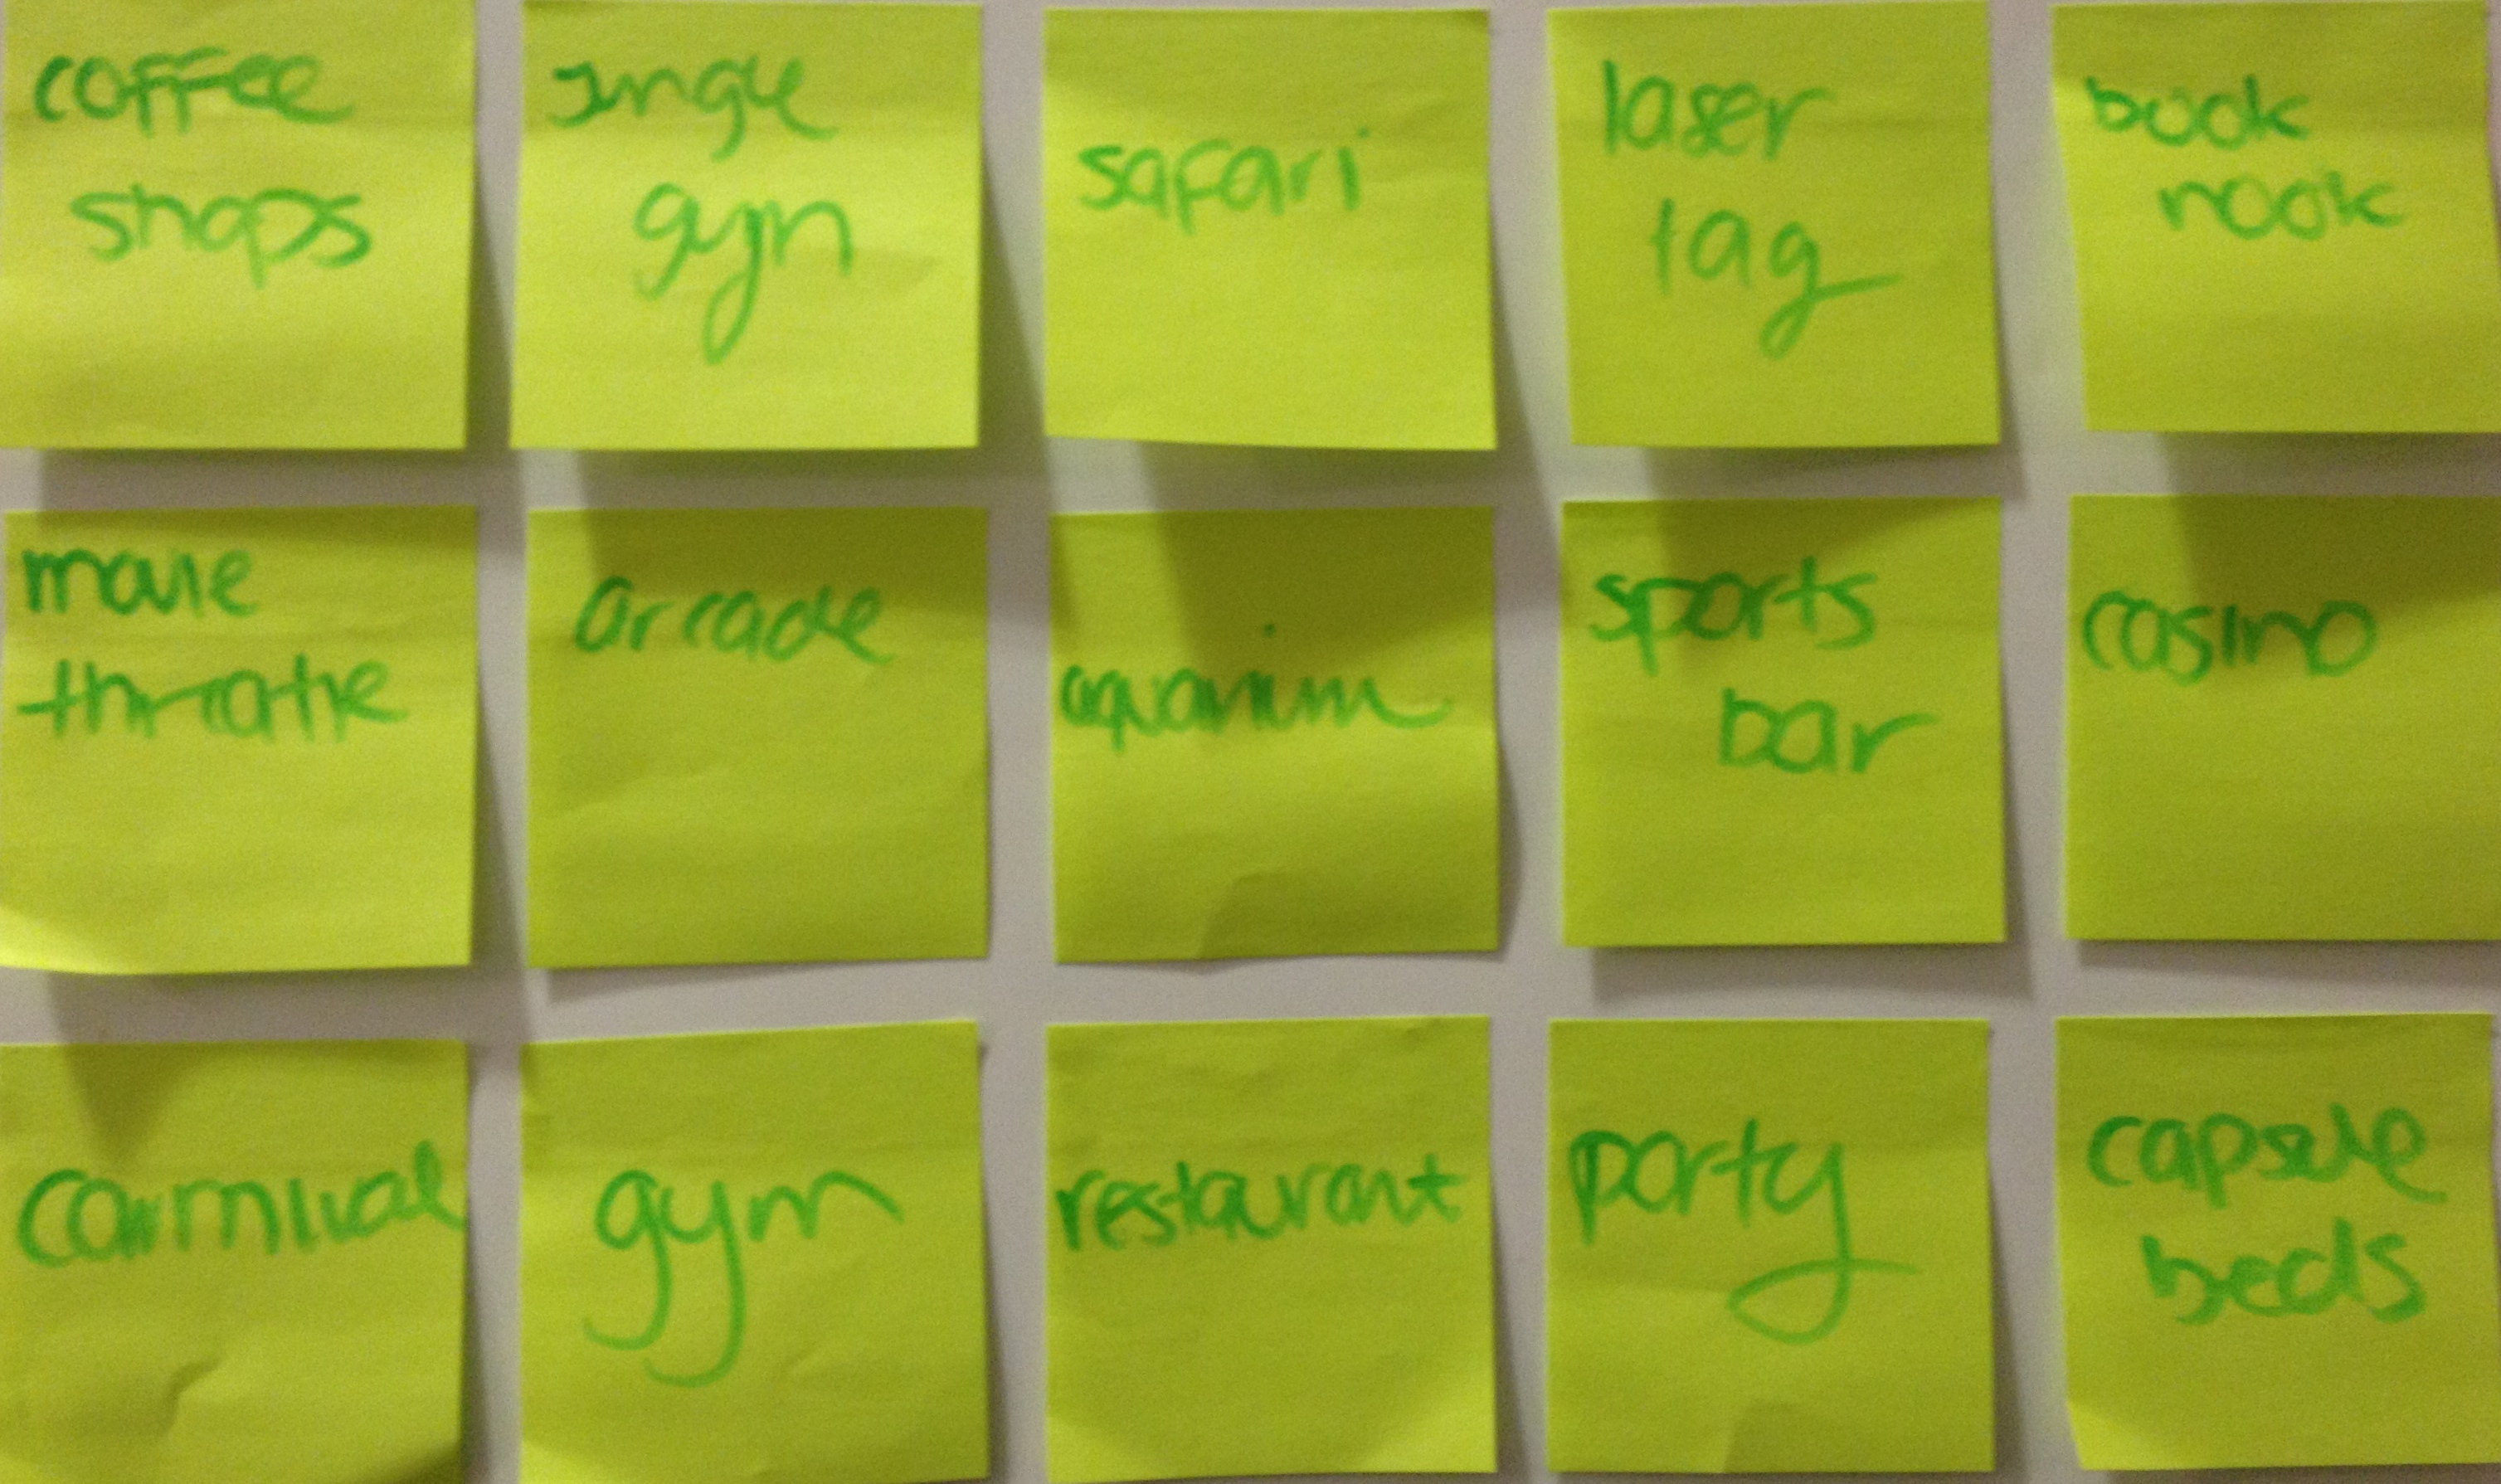
\includegraphics[width=7cm]{DarkHorse/possible_themes.jpg}
   \caption{Possible ideas for a new cabin configuration}
  \label{fig:possible_themes.jpg}
\end{figure}

Our goal for the first Dark Horse Prototype was to find ways to make flying an enjoyable activity, not just another form of transportation. While many passengers find that getting to and around the airport, going through security, and waiting for a flight to board can be a waste of time and a draining activity, people are willing to pay to stand in line at theme parks for hours on end just to get on a fun ride for a few minutes or camp out outside of stores just to get the new iPhone. We believe that if we could make the flying experience a better one, passengers would be less bothered by the less-than-pleasant activities leading up to it. 

We realized that a redesigned cabin would need to be more accessible but could also have different sections explicitly to harness our users? varied needs and reasons for flying. Flying tends to be a time for rest for many and because of this we researched what others had done to convert the cabin from a ?sitting room only? configuration to a more sleep-friendly space. One of the proxies we looked at were the pod hotels in Japan, shown in Figure \ref{fig:hotel_pod.jpg}, where people sleep in fairly compact space-efficient pods. Similar pods could be designed for use in an airplane cabin, reappropriating room typically used for seating to sleeping spaces.

\begin{figure}[h]
  \centering
     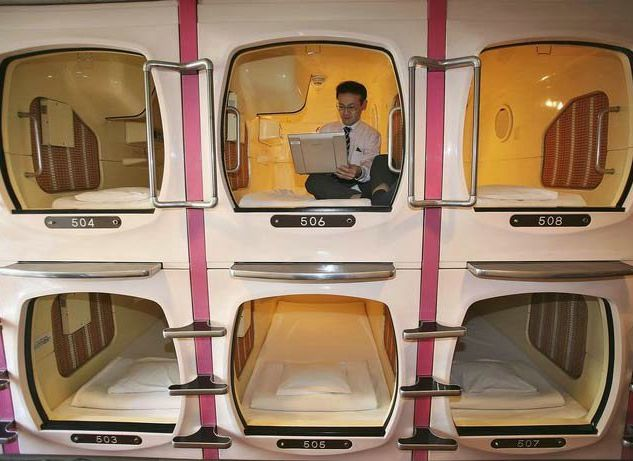
\includegraphics[width=7cm]{DarkHorse/hotel_pod.jpg}
   \caption{Current pod hotel layout in Japan. Source: http://montaraventures.com/blog/2008/06/08/pod-hotel/}
  \label{fig:hotel_pod.jpg}
\end{figure}

There are a number of possible airplane configurations for converting the whole airplane into beds. This could be done by utilizing the vertical space available in the cabin, as shown in Figures \ref{fig:blue_vertical_configuration.png} and \ref{fig:blue_vertical_configuration.png}. 

\begin{figure}[h]
  \centering
     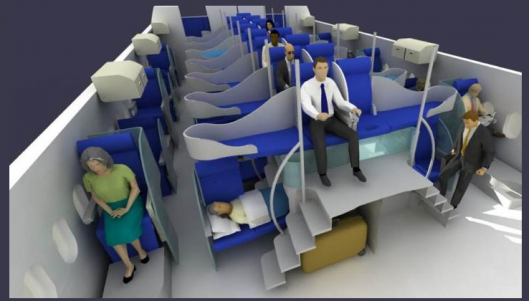
\includegraphics[width=7cm]{DarkHorse/blue_vertical_configuration.png}
   \caption{Example of cabin layout that integrates both chairs and beds and does not decrease the total number of seats. Source: http://www.gizmag.com/future-of-air-travel-comfortable-seating/17751/}
  \label{fig:blue_vertical_configuration.png}
\end{figure} 

\begin{figure}[h]
  \centering
     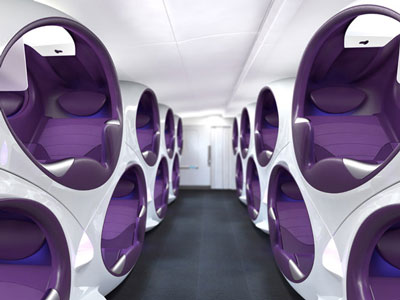
\includegraphics[width=7cm]{DarkHorse/purple_vertical_configuration.png}
   \caption{Example of cabin layout with built in beds. Source: http://www.aviationinsurors.com/chair.html}
  \label{fig:purple_vertical_configuration.png}
\end{figure} 

These configurations make the flying experience much more comfortable while at the same time enabling selective seats to be much more accessible than others. These configurations would allow our users to easily get in and out of their seats without facing the problems they face today.

Our team also explored the possibility of sleeping while standing as opposed to laying down and found that there are several design firms that have been exploring vertical seating arrangements like the one shown in Figure \ref{fig:vertical_seating.jpg}. These designs have received a lot of backlash due to their perceived disregard for passenger comfort despite the fact that they may actually be better for our health. 

\begin{figure}[h]
  \centering
     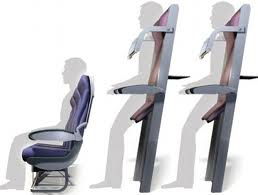
\includegraphics[width=7cm]{DarkHorse/vertical_seating.jpg}
   \caption{Vertical seating being designed for airplane chairs. Source: http://www.dailymail.co.uk/news/article-1215081/Packed-like-sardines-New-aircraft-design-plans-seat-passengers-face-face.html}
  \label{fig:vertical_seating.jpg}
\end{figure} 

We know that many of our users travel for work purposes so we also considered what the best places to comfortably do work are and found that many preferred coffee shops to their offices. Our team also thought about having a gym integrated during the flight, transforming that seemingly lost flight time into a productive workout. Finally, we looked at different products available for creating a more accessible experience, including handles, conveyor belts and revolving doors. From all of this research, we created our first Dark Horse prototypes.
 
\subsection{Description}
In order to make our users think about the present and not only their future destination we wanted to build a flexible and dynamic cabin layout enabling a more customized flight experience for everyone, especially handicapped passengers.

We made the assumption that when passengers buy their tickets, they will have to go through a questionnaire asking them for their preferred activity during the flight. According to their answers they will be placed in the appropriate section of the plane and have the opportunity to do what they really want to do during the flight. If the passengers have special needs due to physical handicaps, we wanted each of our different sections to address these issues and improve the experience not only for everyone, but in particular for those with reduced mobility.  

Our team decided to focus on the design of 5 main sections and built a dynamic scale model for each one:

\textbf{Sleeping area}

We wanted our user to be able to rest and relax so we thought of different types of beds or resting pods as mentioned in the benchmarking section. However, when we tried to prototype them and build our scale model we found at that it was quite hard to keep the number of seats the same. In order to not violate this constraint, our team decided to explore solutions that require a very limited space. As such, we designed our sleeping section with foldable seats which can be unfolded to become a bed as shown on the next picture.

\begin{figure}[h]
  \centering
     \includegraphics[width=7cm]{DarkHorse/PHOTOROBBIE}
   \caption{Plane section dedicated to sleep and relaxation with two configurations: take-off/landing (left) and cruise (right)}
  \label{fig:PHOTO ROBBIE}
\end{figure}

We also studied the possibility of using hammocks but the available space in the cabin was not sufficient to make it work.


\textbf{Family area}

When talking about passengers with reduced mobility people generally picture wheelchair users and passengers with other physical handicaps, but in a sense, families with young children and pregnant women also have reduced mobility compared to the average passenger. In order to address their specific needs our team designed an entire section of the plane to be the family compartment.

We designed this section to be flexible and easily adaptable to family needs. If parents want to sit close to their children and look after them they can get rid of the armrests and convert their row of seats into a sort of bench allowing the family to stay together during the flight. In order to make it easier for parents, children and pregnant women to move through this area we coupled our idea of a bench with the design of a retractable table that can be folded and unfolded between two consecutive rows of seats facing each other. When the table is unfolded it is then easier for people on the benches to access the aisle as shown on the following pictures. 

\begin{figure}[h]
  \centering
     \includegraphics[width=7cm]{DarkHorse/PHOTOROBBIE}
   \caption{Plane section dedicated to family with two configurations: take-off/landing (left) and cruise (right)}
  \label{fig:PHOTO ROBBIE}
\end{figure}

We also considered the fact that the family section of the plane could be sound proof in order to prevent disturbances to the sleeping compartment and concentrate the noise of children playing together in one single area.

\textbf{Gym area}

When our team brainstormed about what people would like to do during their flight we thought that being able to move your limbs and stretch was a big issue, especially for people with blood circulation problems. In order to solve that we thought that having convertible seats that can be turned into yoga mats or that can be used as gym accessories could improve our user?s experience. We imagined a cabin layout that is standard for takeoff and landing but that can be turned into a gym area during the cruise, as displayed in the figures below. 

\begin{figure}[h]
  \centering
     \includegraphics[width=7cm]{DarkHorse/PHOTOROBBIE}
   \caption{Plane section dedicated to sports and physical training with two configurations: take-off/landing (left) and cruise (right)}
  \label{fig:PHOTO ROBBIE}
\end{figure}

People with reduced mobility sometimes need to do physical therapy (PT) exercises to avoid blood circulation issues. However, handicapped people can rarely do their PT exercises alone so it?s possible that flight attends could be trained specifically to assist these passengers.

We also took into account the fact that people are often thirsty due to perspiration when they are physically active so we thought about a system of individual straws that would be available in each passenger?s space allowing to drink water whenever they want without having to call the flight attendants or move across the cabin. This idea can also be extended to all the sections and all the passengers allowing them to feel more in control and more independent.

\textbf{Book Nook}

Since a lot of people, including those with reduced mobility, travel by plane for professional reasons our team wanted to design a plane section that imitates the cosy atmosphere of a coffee shop where people feel relaxed and comfortable while working.
To do so we imagined convertible seats that can be turned into couches and provide better support for people with reduced mobility. 

\begin{figure}[h]
  \centering
     \includegraphics[width=7cm]{DarkHorse/PHOTOROBBIE}
   \caption{Plane section dedicated to work in a cosy atmosphere with two configurations: take-off/landing (left) and cruise (right)}
  \label{fig:PHOTO ROBBIE}
\end{figure}

We also thought that having a round table with one or two flight attendants in the center providing drinks was a good way to have them closer to passengers requiring more attention and assistance.

\textbf{Ease of access - Carousel}

We decided to fully dedicate the last plane section we designed to people with reduced mobility. In the previous sections we addressed their issues by trying to improve everyone experience so that handicapped people would not feel segregated, but for this last section we focused specifically on their needs and expectations. 
Our team found out that boarding and disembarking from the plane and moving in/out of their seats were the biggest issues for passengers with reduced mobility. In order to improve this part of their flight experience, our team decided to get rid of the current cabin layout where seats are lined up. 

We wanted to explore a different configuration where the seats are part of a carousel system that rotates so that any time a passenger enters the aircraft the seat right in front of them is empty. This would limit the distance people have to cover to get to their seat and should make it easier for them to move in/out of their seat since there is no obstacle in front of them as shown in the following pictures.

\begin{figure}[h]
  \centering
     \includegraphics[width=7cm]{DarkHorse/PHOTOROBBIE}
   \caption{Plane section dedicated to people who need easily accessible seats}
  \label{fig:PHOTO ROBBIE}
\end{figure}

We also thought that one of the seats from the carousel could be removed from the circle, making the center of the system accessible. If the central part of the carousel can be accessed then it could be used as a place where wheelchairs or other equipment could be stored.


\subsection{User Feedback and Learnings}

The following learnings came as a result of team discussions, analysis, and feedback from the teaching team. 
It is difficult to reconfigure the cabin without losing seats. However, to maximize profit airlines do not want to lose any seats, making it important to maintain the same number.
The number of possible cabin configurations increase with the implementation of dynamic seats.  Dynamic seats will allow for movement of cabin sections to meet the demands of each passenger. 
Personalizing the flight would improve the experience for all passengers, not just disabled passengers. Many passengers compare the boarding and flight experience to the herding of cattle. By allowing passengers to choose their preffered cabin surrounding or configuration, they play a role in their experience and have more control over their situation. 
Flight attendants may be able to play different roles in the passengers? experiences.  They would be able to cater more toward what a passenger wants instead of performing a wide range of services for all passengers who might not need or want a certain service. 
Every cabin configuration that can be implemented needs to have accessible features to fit the wide range of users our project encompasses.  The new cabin configurations cannot neglect our target user and should not make them feel singled out. 

\section{Dark Horse Version 2}
\subsection{Benchmarking}


Our learnings from version 1 inspired us to continue to explore changing the cabin layout while also putting additional emphasis into the boarding process. We realized that if we could make the seats more accessible, we would be able to alleviate some of the pain brought on by the transfer process into today?s chairs. We looked at cabin configurations like the one in Figure \ref{fig:cabin_against_wall.jpg} where the seats face toward the inside of the cabin as opposed to the front. By having the seat face the passenger, it would be much easier to get in without having to worry about climbing over armrests or other passengers. 

\begin{figure}[h]
  \centering
     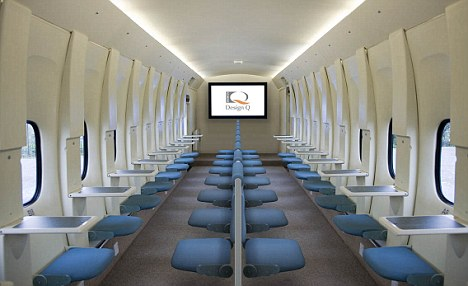
\includegraphics[width=7cm]{DarkHorse/cabin_against_wall.jpg}
   \caption{Vertical seating being designed for airplane chairs. Source: http://www.dailymail.co.uk/news/article-1215081/Packed-like-sardines-New-aircraft-design-plans-seat-passengers-face-face.html}
  \label{fig:cabin_against_wall.jpg}
\end{figure} 

The team researched this further and found that seats are configured to be faced either toward the front or back for safety reasons relating to the forces that passengers could experience during flight. Having seats face inward could subject passengers to excessive lateral forces. Additionally, from the public reception of the configuration shown in Figure \ref{fig:cabin_against_wall.jpg},  we found that passengers would not feel comfortable directly facing other passengers. Thus, we looked at different types of boarding mechanisms that would enable a simpler boarding experience but that would also retain the safety level found in airplanes today. 

\subsection{Description}

In order to solve the problems faced by mobility challenged passengers we tried to radically change the boarding experience for everyone. To this end, our team decided to further investigate carousel concept developed in dark horse version 1 and push it to the extreme.

In order to go as far as possible with this concept we decided to:

 \begin{easylist}[itemize]

& Rethink the whole boarding process from the gate to the seat by creating a carousel inspired by a conveyor belt system through the entire plane.

& Design for an extreme case: a person with no mobility, i.e. a passenger without the use of any limbs. It made our mission more challenging but we thought it could be a good way to make sure we do not overestimate what a people with reduced mobility can or cannot do. In order to reach our goal, we brought a new persona: a mannequin filled with sand to mimic the weight of a real person.

\end{easylist}

We wanted our new persona to go through all the steps of the brand new boarding process we imagined:

\begin{easylist}[itemize]

& Waiting in line at the airport gate where position in the line is determined by seat number. This will facilitate the boarding process since people will have to board in the order defined by the cabin layout. Those in the aft of the plane would go first.

& While waiting, our new persona would be transferred to an airport chair that will then facilitate the transfer to the seat.

& When boarding starts, our persona will use a transfer mechanism located in the front of the cabin to reach his or her seat. Here are different options we modeled:

 \begin{easylist}[itemize]
	& The \textbf{hammock}-type transfer involves a seat that is detachable and can be moved from one chair to another using a lift
\begin{figure}[h]
  \centering
     \includegraphics[width=7cm]{DarkHorse/PHOTOROBBIE}
   \caption{Hammock transfer to enable people to go from the airport chair to their seat}
  \label{fig:PHOTO ROBBIE}
\end{figure} 

	& The \textbf{comb} seat involves two separate pieces which have interlocking teeth; one can be lifted up, bringing the passenger with it, then installed on another chair
\begin{figure}[h]
  \centering
     \includegraphics[width=7cm]{DarkHorse/PHOTOROBBIE}
   \caption{Comb seats that would facilitate the transfer from the airport chair to the seat}
  \label{fig:PHOTO ROBBIE}
\end{figure} 

	& The \textbf{sliding seat} is a seat on rails that can be slid off of one chair and onto another, with the rails collapsing into the chair's body
\begin{figure}[h]
  \centering
     \includegraphics[width=7cm]{DarkHorse/PHOTOROBBIE}
   \caption{Sliding seat allowing people with reduced mobility to reach their seat without assistance}
  \label{fig:PHOTO ROBBIE}
\end{figure} 

\end{easylist}

& Once our user is seated, his seat will then be moved via the carousel/conveyor belt to its standard position as shown on the next drawing.

\begin{figure}[h]
  \centering
     \includegraphics[width=7cm]{DarkHorse/carousel for the dummies.png}
   \caption{Carousel system conveying the seats from the entrance of the plane to their appropriate location}
  \label{fig:Carousel_system}
\end{figure} 

\end{easylist}

\subsection{User Feedback and Learnings}

The learnings for this iteration of dark horse resulted from team discussions, user suggestions and feedback, observations of the user persona, and teaching team feedback. 
The transfer mechanism to move the user into the airplane chair is still a problem that needs to be addressed. The user has to be able to make it from the waiting lounge to the airplane seat with the feelings of control, comfort and stability. 
The experience prototype of boarding did not include a mechanism to deal with luggage. The process of storing and carrying luggage needs to be addressed within the prototype to represent the entire experience. 
Communication is key to allow our users to feel comfort, safe, and stable within the new process. The process needs to be communicated effectively and sufficiently to allow for our users to have a better experience and to feel as if this process is better than the previous boarding process. 
Users want to be able to worry and stress less about getting to their seats and finding a place for their luggage. The new boarding process would allow the users to use the boarding time on a more enjoyable pastime. 
The users have to exert less effort with this boarding process because boarding is automated and does not require the need to locate their seats and maneuver the aisle. 
Our user was concerned with bumping into objects or other seats or hitting the wall during movement. The boarding process needs to be done in such a way that the users and passengers feel safe and secure with the movement and with process as a whole.  Lateral accelerations need to be considered to create a smooth ride and efficient boarding process. 
Sensors would need to be implemented into a functional prototype or a mechanical prototype to simulate the actual boarding process by having the interim stops to board new passengers.  Sensors would also need to be implemented into the process to prevent collisions or accidents in the case of a malfunction. 

\section{Dark Horse Version 3}

\subsection{Benchmarking}

During our user testing for our second version of the Dark Horse prototype, we realized carry-on luggage was a huge concern. Currently, luggage is stored in a very burdensome and unintuitive way and with version 3 we sought out to redesign the carry-on luggage experience. 
Our users have voiced their concerns about not being able to store/reach their luggage as well as the panic they feel when they are not aware of where their belongings are being stored. Our team looked at a couple of different designs out there that use the vertical space within the airplane in a different manner to accommodate both people and luggage in a more user friendly way. 

\begin{figure}[h]
  \centering
     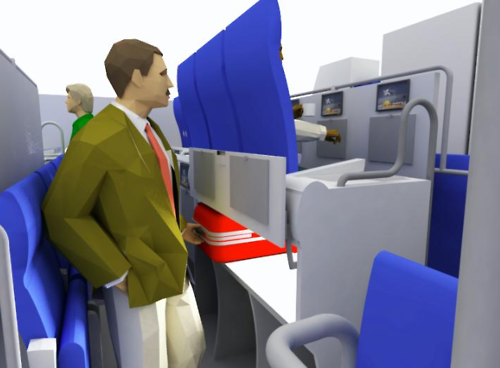
\includegraphics[width=7cm]{DarkHorse/luggage_trays.png}
   \caption{Design that allows for easier luggage storage for all passengers Source: http://www.gizmag.com/future-of-air-travel-comfortable-seating/17751/}
  \label{fig:luggage_trays.png}
\end{figure}  

The design shown in Figure \ref{fig:luggage_trays.png} displays a cabin layout where consecutive rows of seats are on different levels, allowing passengers to store their luggage behind their tray but under the seat of the person in front of them. This design puts luggage at the ideal height for both standing and sitting passengers as depicted by the image in Figure \ref{fig:correct_height.png}, a standard design rule for access and mobility.  

\begin{figure}[h]
  \centering
     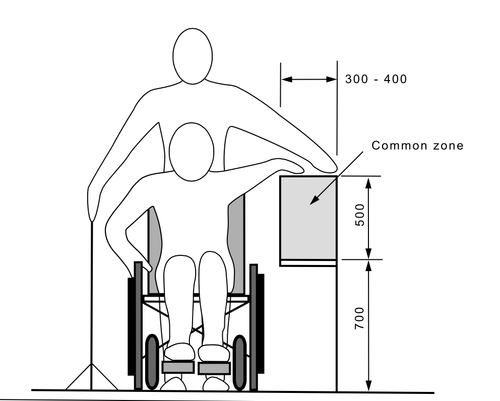
\includegraphics[width=7cm]{DarkHorse/correct_height.png}
   \caption{Ideal height for reaching objects for both sitting and standing passengers. Source: https://law.resource.org/pub/nz/ibr/nzs.4121.2001.svg.html}
  \label{fig:correct_height.png}
\end{figure} 

Another design solution we explored was actually having two seats on top of each other as shown in Figure \ref{fig:vertical_with_luggage.jpg}. This design opens up the area under the stairs for luggage storage, which could also include a passenger?s wheelchair, allowing for a less stressful flying experience for handicapped users. The bed next to the seat could also be used to provide passengers flying with toddlers with extra room to put them in so that they do not have to sit on their lap throughout the whole flight. 

\begin{figure}[h]
  \centering
     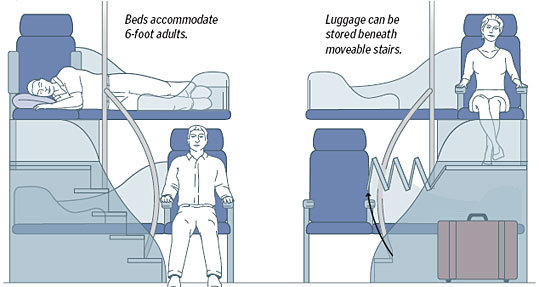
\includegraphics[width=7cm]{DarkHorse/vertical_with_luggage.jpg}
   \caption{Vertical cabin configuration with luggage storage Source: http://www.boston.com/business/articles/2009/06/15/taking_airline_seat_configurations_vertical/}
  \label{fig:vertical_with_luggage.jpg}
\end{figure} 
transfer

Another main concern for our user was the actual transfer process and how they would get from an aisle chair to their seat. We know that today people can use transfer boards, they can be carried by someone else or, if they are strong enough, they can transfer themselves. We found that there are some products on the market that could make the transfer experience better, such as the ?harness? shown in Figure \ref{fig:harness.jpg} or the walker in Figure \ref{fig:walker.jpg}. We believed that the walker would be an interesting solution if we were able to add mechanisms  that would lower the bar supporting the person?s weight to get it closer to the seat and that would swing the blue supports open such that the person would come in contact with the chair. Eventually, we actually decided to widen the airplane aisle and get rid of the transfer all together. 

\begin{figure}[h]
  \centering
     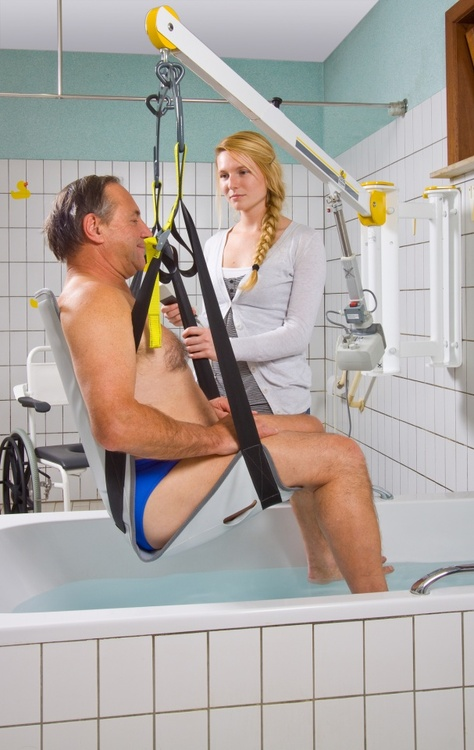
\includegraphics[width=7cm]{DarkHorse/harness.jpg}
   \caption{Harness used to get disabled out of the bath. Source: http://www.handimove.com/en/products/bath-seat-pvc/}
  \label{fig:harness.jpg}
\end{figure} 
transfer

\begin{figure}[h]
  \centering
     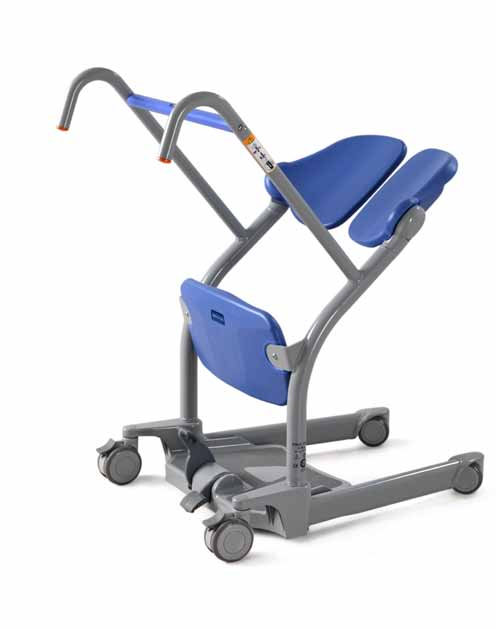
\includegraphics[width=7cm]{DarkHorse/walker.jpg}
   \caption{Walker that could be adapted to become a better aisle chair. Source: http://mobilityexpress.com/Sara-Stedy-Seated-Transfer-Device_1154.htm}
  \label{fig:walker.jpg}
\end{figure} 
transfer


\subsection{Description}

Currently, people with reduced mobility have to first transfer from their own wheelchair to the aisle wheelchair which is uncomfortable and narrow. Once boarding starts, the user is brought to his/her seat by a flight attendant or an airline employee and is then transferred to his/her seat. This process is long, it puts people with reduced mobility apart by making them different and it deprives them from their independence because the aisle wheelchair must be maneuvered by a flight attendant. Therefore, since the boarding process is such a pain point for our users we decided to work on it to improve their experience and give them more independence.

During the boarding process the two steps that are critical for our users are :

 \begin{easylist}[itemize]

& First, the access to their seats. Our team thought that if we could enable people with reduced mobility to enter the aircraft with their own wheelchair and then give them the possibility to transfer themselves from their wheelchair to their seat without someone else helping them it would considerably improve their experience.

& Second, the luggage storage. People with reduced mobility frequently cannot access the luggage compartment because it is too high, so our team thought that if we could imagine a system that makes the luggage compartment go up and down by just pressing a button it would also contribute to make the flight experience better for people with reduced mobility.

\end{easylist}

\textbf{Helping our user access his/her seat}

Our objective was to enable passengers to enter the aircraft with their own wheelchair and to do so we had to figure out a way to make the aisle wider. Initially we did not want to take into account the constraint of keeping the number of seats in the aircraft the same so we imagined a new cabin layout for boarding. The idea was to have the aisle seats on rails so that they could be moved and lined up with the window seats as shown in Figure \ref{fig:first_new_cabin_layout} . 

\begin{figure}[h]
  \centering
     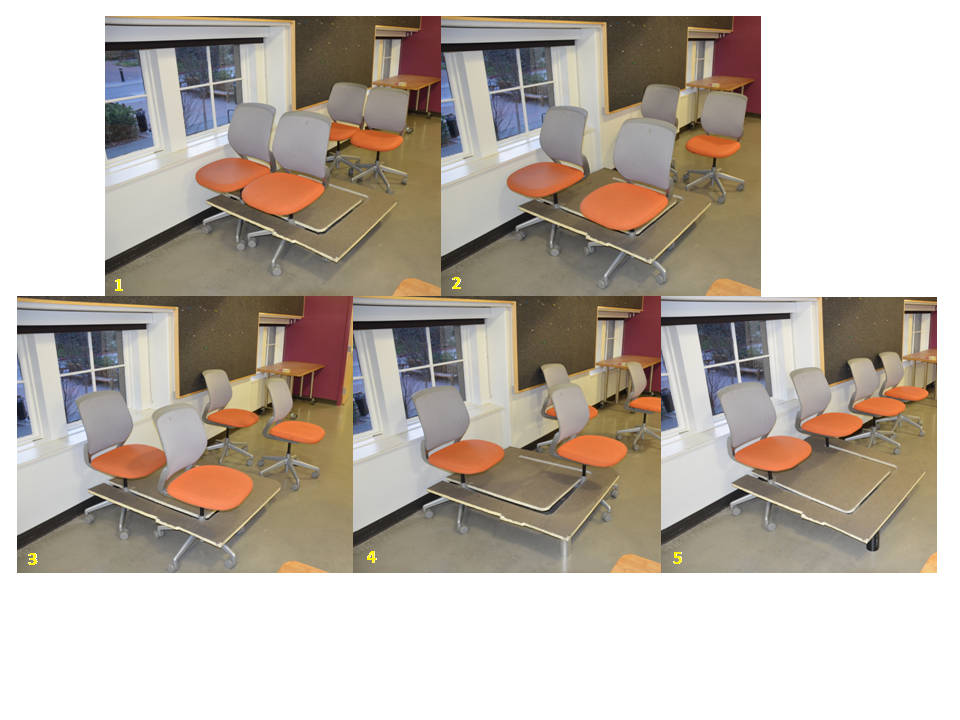
\includegraphics[width=7cm]{DarkHorse/first_new_cabin_layout.jpg}
   \caption{Our first new cabin layout for boarding the plane}
  \label{fig:first_new_cabin_layout}
\end{figure} 

With this system all the seats would be lined up on each side of the plane and the aisle during the boarding process would then be three times bigger than in flight, allowing people with reduced mobility to enter the aircraft with their own wheelchair which is on average 30?? wide, as shown in Figure \ref{fig:wheelchair_dimensions} .

\begin{figure}[h]
  \centering
     \includegraphics[width=7cm]{DarkHorse/wheelchair dimensions.jpg}
   \caption{Standard wheelchair dimensions}
  \label{fig:wheelchair dimensions}
\end{figure}

But we realized that with this system it was impossible to keep the total number of passengers on board the aircraft the same because the proposed boarding layout requires too much space per seat. 

Therefore, we thought of a second cabin layout for the boarding process which also makes the aisle wider but in a more reasonable way. We looked at the dimensions of a standard Embraer plane (Figure \ref{fig:embraer_plane} ) and found out that if we were able to angle the rows by 46.2� (see Figure \ref{fig:angled_seats}) from their current position we could make the aisle wide enough (42.87??) to enable our passengers to reach their seats in their own wheelchair while keeping the total number of seats the same.

\begin{figure}[h]
  \centering
     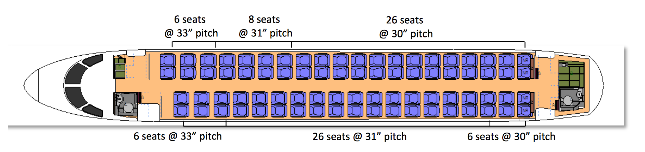
\includegraphics[width=7cm]{DarkHorse/embraer_plane.jpg}
   \caption{Standard Embraer plane cabin layout}
  \label{fig:embraer_plane}
\end{figure}

Our concept was to initially have all of the rows of the plane linked to a mechanism that would rotate the seats before the boarding process, making a wider aisle for passengers. Passengers with reduced mobility who have reached their seats with their own wheelchair would be able to transfer to their plane seats. If they are strong enough they may be able to transfer themselves without requesting flight attendants assistance, but if they need help we imagined that they could use one of the transfer mechanisms mentioned in the benchmarking section.
\begin{figure}[h]
  \centering
     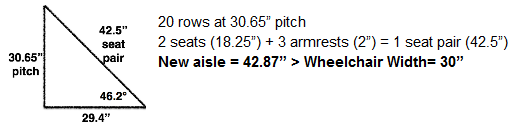
\includegraphics[width=7cm]{DarkHorse/angled_seats.jpg}
   \caption{New cabin layout with angled seats for boarding}
  \label{fig:angled_seats}
\end{figure}

Once the passengers are all seated (potentially while the aircraft is taxiing towards the runway) the seats would go back to the standard non angled cabin configuration for take off and would remain in that state for the duration of the flight. When the plane stops at the gate and is ready for passengers to disembark, the seats would be angled again and flight attendants would bring passengers with reduced mobility their own wheelchair so that they would be able to leave the plane on their own. 

\textbf{Helping our user accessing the luggage compartment}

We found out that accessing the seat is not the only problem disabled people are confronted with: they also have a big issue when they want to store their personal items in the luggage compartment. In order to fix this, our team designed a luggage compartment that can go up and down on demand, controlled by our user pressing a button (Figure \ref{fig:embraer_plane}).

\begin{figure}[h]
  \centering
     \includegraphics[width=7cm]{DarkHorse/our_luggage_compartment.jpg}
   \caption{Our luggage compartment which is accessible on demand by pressing a button}
  \label{fig:our_luggage_compartment}
\end{figure}

In order to build this system we designed a mechanism made of rope and pulleys that is inspired from systems used to stabilize cameras that are mounted on drones and model aircraft. While piloting the system that causes the camera to move, the device has to remain stable. This mechanism avoids the creation of moments that could cause the ropes to tangle and knot. For our system we wanted to have a luggage compartment that does not experience torques and that can come up and down in the most smooth and stable way.

\subsection{User Feedback and Learnings}

Several classmates and peers were users for this prototype and provided the majority of our learnings.  However, some of the learnings came directly from team observations during user testing. The learnings are divided into the reconfiguration and the luggage. 
Reconfiguration: 
Our testing revealed that the users were concerned about what would happen to their feet during the transformation of angled seating to the regular configuration and vice versa.  Some users suggested the addition of a footrest.  But where would the ideal location be? This revelation is very important to our target users because some of them do not have the ability to move their legs out of the way or to move with the chair.  This would also mean they would have to manually put their feet on a footrest, and the ideal position of the footrest would need to be designed to help the target users have a better experience.
A single, continuous rotation mechanism would be better than multiple discrete for all passengers.  The users commented that the mechanism should be similar to the movement of a car seat because it is slow enough and does not cause a great amount of force and acceleration to be placed on the passenger. In addition, the window seat experienced less movement or felt like it experienced less movement than the aisle seat.  This is important due to the benchmarking findings of last quarter that showed that the target users preferred the window seat over the aisle seat. 
Passengers would be able to board faster due to a wider aisle that allows for easier maneuvering of the cabin space.  The wider aisle would allow for a double line of traffic to head down the aisle instead of one line. 
The wider aisle would allow for a wheelchair to be able to maneuver down the aisle to the seat.  The wheelchair would have tolerances on both sides as it moves down the aisle to allow for a comfortable fit.  It would be easier for a mobility challenged passenger to get into the aisle seat but to access the window a handle may be needed. 
The legroom is the limiting factor with the reconfiguration.  When the seats are in the angled arrangement, the window seats have less legroom than in the normal configuration.  The angle of the seats would need to be reconfigured to allow for a smaller angle with more legroom but still create a wider aisle with plenty of tolerance for a wheelchair. However, it was noted that it is easier to board and disembark with angled seats.  Thus, angled seats would be the preferred configuration for boarding and disembarking from the plane. 
It may be possible to achieve the desired effect by only rotating several of the aisles, allowing increased access to those seats specifically.
Luggage: 
The luggage bin needs to move with the seats into the angled configurations. With the bins situated parallel to the normal cabin configuration when the seats are angled, it is difficult to load the luggage into the bin without awkward movements. 
The luggage bin should be lowered to arm level instead of head or face level.  Users felt claustrophobic when the bin was at head level due to the reduction in vision. The bin was in the line of sight which made it uncomfortable and a very closed-off space.  
The bin should have a door and have a slightly steeper angle or have a lip. Luggage moves during flight due to turbulence and shifting due flight. This would prevent luggage falling out on the passengers or items being broken. 
A more rigid lowering mechanism needs to be used instead of the string and rope mechanism that was used during prototyping.  Users did not feel that the bin was stable and looked scared as it was lowered down.  They feared the bin might move during lowering, raising, or turbulence causing it to hit them or bring their belongings.  
More research for optimal lowering position needs to be conducted.  The position that we prototyped did not receive good feedback from the users.  Therefore, several iterations need to be performed to see what would be best for our target users and other passengers
Most of the users wanted to store luggage before they sat in their seat.  The orientation of the bin and the height of the bin makes this a very awkward and uncomfortable task.  When the users sat with their luggage, they felt that they were crowded and did not know what to do with the luggage until the bin was available.  The mechanism to raise and lower the bin needs to be fast and stable to allow for ease of access to the seat and aisle depending on the activity.
\end{document)
